\chapter{Geometric phase effect\label{app:GPE}}

\section{Geometric phase effect as a Bloch-Siegert shift}

Experiments designed to measure the Electric Dipole Moment~(EDM),
typically observe particles of interest as they move through a region
of uniform and aligned $\vec{E}$ and $\vec{B}_0$ fields. The
particles under question are usually neutral and have a total spin
angular momentum $\vec{J}$. The external field interaction
Hamiltonian is
%
\begin{equation}
H_{ext} = \frac{\mu_a}{J}\vec{J}\cdot\vec{B}_0 - \frac{d_a}{J}\vec{J}\cdot\vec{E},
\end{equation}
%
where $\mu_a$ and $d_a$ are the magnetic and electric dipole moments,
respectively.
The Larmor precesssion frequencies, for parallel and antiparallel
$\vec{B}_0$ and $\vec{E}$, are given by the expressions
%
\begin{equation}
\label{eqn:GPEw}
\omega_{L\uparrow\uparrow} = -\frac{(\mu_a B_{0\uparrow\uparrow} + d_a E)}{J\hbar} \; , \; \omega_{L\uparrow\downarrow} = -\frac{(\mu_a B_{0\uparrow\downarrow} - d_a E)}{J\hbar} 
\end{equation}
%
An EDM will reveal itself by causing a reduction or enhancement of the
accumulated precession frequency according to whether the fields are
parallel or anti-parallel.

If the particles are moving through static, but non-uniform fields,
there exists motion of the fields in the frame of any particle.  This
causes geometric phases~(GP's) in the precession of the total spin of
the ensemble, which is generally independent of the precession caused
by an EDM. Therefore, the terms $+\epsilon_{geo\uparrow\uparrow}/T$
and $+\epsilon_{geo\uparrow\downarrow}/T$ should be added to the
right-hand sides of Equations \ref{eqn:GPEw} respectively.  The
accumulated phase measured int he time interval $T$ will be
%
\begin{equation}
(|\omega_{L\uparrow\uparrow}| - |\omega_{L\uparrow\downarrow}|)T = \frac{|\mu_a|(B_{0\uparrow\uparrow} - B_{0\uparrow\downarrow})T}{J\hbar} \pm \frac{2 d_{a} E T}{J \hbar} \pm (\varepsilon_{geo\uparrow\uparrow} -\varepsilon_{geo\uparrow\downarrow}) \;,
\end{equation}
%
where the sign alternative has to be chosen to be the same as the sign
of $\mu_a$.  If $B_0$ remains constant while $\vec{E}$ is reversed,
then the first term becomes zero. The geometric phase term will result
in a false EDM $d_af$ given by
%
\begin{equation}
\label{eqn:daf}
d_{af} = -(\varepsilon_{geo\uparrow\uparrow} -\varepsilon_{geo\uparrow\downarrow})\frac{J\hbar}{2 E T} = -(\Delta \omega_{geo\uparrow\uparrow} - \Delta \omega_{geo\uparrow\downarrow})\frac{J\hbar}{2E} \; ,
\end{equation}
%
where $\Delta \omega_{geo\uparrow\uparrow}$ is the average rate of
accumulation of the GP proportional to $E$ for the particle ensemble
of spins in parallel fields.

As a particle moves through the electric field with velocity $v$, it
experiences an effective magnetic field
%
\begin{equation}
\label{eqn:Bv}
\vec{B}_v = \frac{\vec{E} \times \vec{v}}{c^2} \;\;,
\end{equation}
%
which interacts with the particles magnetic moment $\mu_a$, creating a
geometric phase.  This is independent of the interaction of a genuine
EDM with the $\vec{E}$ field.
%
A gradient $\partial B_{0z}/\partial z$, in the case of cylindrical
symmetry, has the associated components in the xy plane,
%
\begin{equation}
\label{eqn:Bxy}
\vec{B}_{0xy} = \vec{B}_{0r} = - \left( \frac{\partial B_{0z}}{\partial z} \right) \frac{\vec{r}}{2} \;\; ,
\end{equation} 
%
at all radial positions $\vec{r}$ relative to the axis of symmetry.

A geometric phase is caused by the combination of $\vec{B}_v$ and
$\vec{B}_{0xy}$, thus
%
\begin{equation}
\vec{B}_{xy} = (\vec{B}_{0xy} + \vec{B}_v) .
\end{equation}
%
These fields are varying with position in the trap.  Here it is
assumed that inhomogeneities in $\vec{E}$ are small enough that they
only effect $\vec{B}_v$ to second order, and thus they will not be
considered.

The particles are assumed to be moving in conditions where
$m c^2 \gg m v^2 \gg |\mu_a B_0|$.  Thus, no relativity is needed
other than Eqn.~\ref{eqn:Bv}.


%We can rely entirely on classical methods to calculate te spin motion using the Bloch equations
%
%\begin{equation}
%d \vec{S} =\frac{\mu_a}{S\hbar}[\vec{S} \times (\vec{B}_v + \vec{B}_0)]dt \; .
%\end{equation}
%
%where we can define $(\mu_a/S\hbar) = \gamma$.
%

Ramsey considered a neutral particle with spin and magnetic moment
precessing with an angular velocity
$\omega_L = \omega_0 = -\gamma B_{0z}$ in a constant magnetic field
$\vec{B}_{0z}$ and the addition of a magnetic field of strength
$B_{xy}$ in the xy plane rotating in the plane at angular velocity
$\omega_r$.  He found that, the Larmor precession frequency $\omega_L$
is shifted away from $\omega_0$, and to first order, this shift
$\Delta \omega = \omega_L - \omega_0$ is given by
%
\begin{equation}
\Delta \omega = \frac{\omega_{xy}^2}{2(\omega_0 - \omega_r)} \;\; ,
\end{equation}
%
where $\omega_{xy} = -\gamma B_{xy}$ ~\cite{ramsey1955}. Here this is
refered to as the Ramsey-Bloch-Siegert ~(RBS) shift.  It is useful to
note that the numerator $\omega_{xy}^2$ is
%
\begin{equation}
\omega_{xy}^2 = \gamma^2 \vec{B}_{xy}^2 =\gamma^2(\vec{B}_{0xy}^2 + \vec{B}_{v}^2 + 2 \vec{B}_{0xy}\cdot\vec{B}_{v}) .
\end{equation}
The first term takes into account the influence of $\vec{B}_{xy}$ on
$\omega_L$ in the absence of an $\vec{E}$ field.  The second term is
proportional to $(\vec{E}\times\vec{v})^2$, and is involved in the
calculation of the second order $(\vec{E}\times\vec{v})$ shift.  The
third term is the one that causes the GP shifts linear in $E$.

\begin{figure}[h!]
\label{fig:trap}
  \centering
    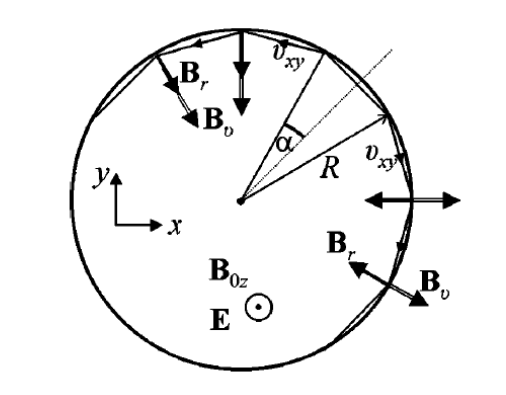
\includegraphics[width=.5\textwidth]{trap.png}
    \caption{Effective magnetic field in the rotating coordinate system}
\end{figure}

Consider a particle in a cylindrical storage vessel with the shape
shown in Fig.~\ref{fig:trap}.  The $z$ axis points along the cylinder
axis of the trap.  Circular electrodes in the $xy$ plane form the roof
and floor of the trap, and the walls are fully specular in terms of
reflections of particles.  It is also assumed that there is no
particle-particle collisions.

It can also be assumed that the particle's motion is confined to the
$xy$ plane with velocity $v_{xy}$, since any motion in the $z$
direction does not contribute to the GP's under investigation
($\vec{E} \times \vec{v} = 0$). The $\vec{B}_0$ field is taken to be
nearly uniform with a small gradient $\partial\vec{B}_{0z}/\partial z$
that is to first order independent of position.  As in~\ref{eqn:Bxy},
also
%
\begin{equation}
\vec{B}_{0xy} = \vec{B}_{0r} = - \frac{\partial B_{0z}}{\partial z} \frac{\vec{r}}{2} = B_{0r} \frac{\vec{r}}{r} .
\end{equation}
%
Very close to the wall of the trap, $\vec{B}_{0r}$ and $\vec{B}_{v}$
are nearly parallel and aligned with the radius $\vec{r}$.  Therefore,
a particle moving along the edge of the trap experiences rotating
radial magnetic field of amplitudes
%
\begin{equation}
\textrm{for} \; \vec{B}_{0 \uparrow} \; \textrm{and} \;\; 
\vec{E}_{\uparrow}, \;\; B_{xy +} = B_{0r} - |B_{v}|, 
\;\; B_{xy -} = B_{0r} + |B_{v}| ~,
\end{equation}
and 
\begin{equation}
\textrm{for} \; \vec{B}_{0 \uparrow} \; \textrm{and} \;\; 
\vec{E}_{\downarrow}, \;\; B_{xy +} = B_{0r} + |B_{v}|, 
\;\; B_{xy -} = B_{0r} - |B_{v}| ~,
\end{equation}
%
where the (+) case is the sense with the particles angular momentum
vector parallel to $\vec{B}_0$ and the (-) case is the opposite sense.
This peripheral motion has $|\omega_r| = v_{xy}/R$, where $R$ is the
trap radius.  As a result,
\begin{equation}
\label{eqn:relations}
|B_v| = \frac{|v_{xy}||E|}{c^2}, \; |\omega_0| = |\gamma B_{0z}|, \; |\omega_r| = \frac{|v_{xy}|}{R},
\end{equation}
%
\begin{equation*}
B_{0r} \rightarrow \lbrace B_{0R} = - \frac{\partial B_{0z}}{\partial z} \frac{R}{2} \rbrace \;\; \textrm{as} \;\; \alpha \rightarrow 0 \; .
\end{equation*}
%
These rotating fields induce shifts in the Larmor frequency, which is
described by the RBS shift equation.  In mechanical equilibrium, any
particle is equally likely to move in either direction around the
trap. To get the ensemble average shift, the shifts of the two senses
of circulation are equally weighted giving
%
\begin{equation}
\Delta \omega = \frac{(\gamma B_{xy+})^2}{4(\omega_0 - |\omega_r|)} + \frac{(\gamma B_{xy-})^2}{4(\omega_0 + |\omega_r|)} .
\end{equation}
%
Inserting the expressions for $B_{xy\pm}$ gives
%
\begin{equation}
\begin{split}
\Delta \omega_{\uparrow\uparrow} = & \frac{\gamma^2 (B_{0R}^2 + B_{v}^2)}{4} \left[ 
\frac{1}{(\omega_0 - |\omega_r|)} + \frac{1}{(\omega_0 + |\omega_r|)} \right] \\ & - \frac{\gamma^2 B_{0R} |B_v|}{2} \left[ 
\frac{1}{(\omega_0 - |\omega_r|)} - \frac{1}{(\omega_0 + |\omega_r|)} \right] \; ,
\end{split}
\end{equation}
%
\begin{equation}
\begin{split}
\Delta \omega_{\uparrow\downarrow} = & \frac{\gamma^2 (B_{0R}^2 + B_{v}^2)}{4} \left[ 
\frac{1}{(\omega_0 - |\omega_r|)} + \frac{1}{(\omega_0 + |\omega_r|)} \right] \\ & + \frac{\gamma^2 B_{0R} |B_v|}{2} \left[ 
\frac{1}{(\omega_0 - |\omega_r|)} - \frac{1}{(\omega_0 + |\omega_r|)} \right] \; .
\end{split}
\end{equation}
%
And taking their difference gives
%
\begin{equation}
\label{eqn:omegadiff}
\begin{split}
(\Delta \omega_{\uparrow\uparrow} - \Delta \omega_{\uparrow\downarrow}) & =   -\gamma^2 B_{0R} |B_{v}| \left[ \frac{1}{(\omega_0 - |\omega_r|)} - \frac{1}{(\omega_0 + |\omega_r|)} \right]
\\ \\ & = -2\gamma^2 B_{0R} |B_{v}|\frac{|\omega_r|}{(\omega_0^2 - \omega_r^2)}\; ,
\end{split}
\end{equation}
%
The Eqn.~\ref{eqn:omegadiff} shows that only the cross terms involving
$B_{0R}|B_v|$ contribute to the GP that is linear in $E$.  The factor
$(\omega_0^2 - \omega_r^2)^{-1}$ has a sharp peak and changes sign at
the boundary between the ranges $|\omega_r| < |\omega_0|$ and
$|\omega_r| > |\omega_0|$.

Typical nEDM measurements using UCN work in the nearly adiabatic
regime where $|\omega_r| < |\omega_0|$.  In this case,
Eqn.~\ref{eqn:omegadiff} could be written as
%
\begin{equation}
(\Delta \omega_{\uparrow\uparrow} - \Delta \omega_{\uparrow\downarrow}) = -2\gamma^2 B_{0R} |B_{v}| \frac{|\omega_r|}{\omega_0^2} \left[1-\frac{\omega_r^2}{\omega_0^2}\right]^{-1} \;.
\end{equation}
%
Comparing this with
$(\Delta \omega_{geo\uparrow\uparrow} - \Delta
\omega_{geo\uparrow\downarrow})$ from Eqn.~\ref{eqn:daf}, and using
the relations in Eqn.~\ref{eqn:relations} gives
%
\begin{equation}
d_{af} = -\frac{J \hbar}{2} \left( \frac{\partial B_{0z} / \partial z}{B_{0z}^2} \right) \frac{v_{xy}^2}{c^2} \left[1-\frac{\omega_r^2}{\omega_0^2}\right]^{-1} \; ,
\end{equation}
%
for particles moving in peripheral orbits.

%%%%%%%%%%%%%%%%%%%%%%%%%%%%%%%%%%%%%%%%%%%%%%%%%%%%%%%%%%%%%%%%%%
\subsection{T1,T2, GPE redux}

An alternative approach to determining the geometric phase effect
provides a more general theory, valid for an arbitrary shape of the
magnetic field as well as for arbitrary geometry of the confinement
cell \cite{pignol2012electric}.

The frequency shift induced by a fluctuating transverse field is given
by the Lamoreaux-Golub expression \cite{LamGol2005}:
%
\begin{equation}
\delta \omega = \frac{1}{2}\int_{0}^{\infty}d\tau \cos(\omega_0 t) \langle\omega_x(0) \omega_y(\tau) - \omega_y(0) \omega_x(\tau)\rangle + \frac{1}{2}\int_{0}^{\infty}d\tau \sin(\omega_0 t) \langle\omega_x(0) \omega_x(\tau) - \omega_y(0) \omega_y(\tau)\rangle ,
\end{equation}
%
where the bracket refers to the ensemble average of the quantity of
particles in the trap.

We can write the frequency shift in powers of the magnetic and electric field:
%
\begin{equation}
\delta \omega = \delta \omega_{B^2} + \delta \omega_{E^2} + \delta \omega_{BE}.
\end{equation}
%
If we flip the direction of the electric field, only the linear term in E 
%
\begin{equation}
\label{eqn:deltawBE}
\delta \omega_{BE} = \frac{\gamma^2 E}{c^2} \int_{0}^{\infty} d\tau \cos(\omega_0 \tau) \langle B_x(0) v_x(\tau) + B_y(0) V_y(\tau)\rangle
\end{equation}
%
generates a frequency shift (as long as the field amplitude doesn't
change).  Therefore, it generates a false EDM of:
%
\begin{equation}
d_{False} = \frac{\hbar}{4E}[\delta \omega(E) - \delta \omega (-E)] = \frac{\hbar}{4E}\delta \omega_{BE}(E) ,
\end{equation}
%
The frequency shifts $\delta \omega_{B^2}$, $\delta \omega_{E^2}$, and
$\delta \omega_{BE}$ involve Fourier transforms (evaluated at the
Larmor frequency) of correlation functions involving field and
velocity components.  In the adiabatic regime these can be expanded in
perturbation series using integration by parts:
%
\begin{equation}
\int_{0}^{\infty} d\tau \cos(\omega_0 \tau)\langle B_x(0) v_x(\tau)\rangle = [\cos(\omega_0 \tau)\langle B_x(0)x(\tau)\rangle]_{0}^{\infty} + \omega_0 \int_{0}^{\infty} d\tau \sin(\omega_0 \tau)\langle B_x(0) x(\tau)\rangle ,
\end{equation}
%
where the second term vanishes in the nonadiabatic limit
($\omega_0 \tau_c \ll 1$).  Using this expansion with
Eqn.\ref{eqn:deltawBE}, we arrive at a false EDM:
%
\begin{equation}
d_{False} = - \frac{\hbar \gamma^2}{2 c^2} \langle x B_x + y B_y \rangle,
\end{equation}
%
which is valid for arbitrary field inhomogeneities in the nonadiabatic
regime.


\subsection{Why is it called a geometric phase?}

In the nEDM experiment, it is important to understand how UCN move
adiabatically through a magnetic field gradient.  In the frame of
reference of the UCN, the magnetic field is changing with time, which
results in a Berry phase shift as the particle moves through a closed
curve.  Since the UCN is moving slowly with respect to the change in
magnetic field, its spin will follow the field adiabatically.  The
change in field strength with time is then reflected in the geometry
of the container that the UCN are moving in, and therefore the phase
accrued is geometric in origin.
 

\subsubsection{Adiabatic Approximation}
Consider a Hamiltonian that depends on some set of parameters. If
these parameters change ``slowly" with time, then the energy
eigenvalues will also change as the parameters themselves change. By
slowly, we mean that the parameters change on a time scale T that is
much greater than $\frac{2\pi \hbar}{E_{ab}}$ for some difference
$E_{ab}$ in energy eigenstates.

Starting from the eigenvalue equation for Hamiltonian :
%
\begin{equation}
\label{eqn:Hamiltonian-eigenkets}
H(t)  |n;t\rangle = E_n(t) |n;t\rangle ,
\end{equation}
the Schr\"{o}dinger equation can be written as
%
\begin{equation}
\label{eqn:alpha-schrodinger}
i \hbar \frac{d}{dt} |\alpha ; t \rangle = H(t) |\alpha ; t\rangle .
\end{equation}
%
We can write $|\alpha;\rangle$ in terms of Hamiltonian eigenkets
%
\begin{equation}
\label{eqn:alpha-ket}
|\alpha;t\rangle=\sum_n c_n(t) e^{i \theta_n(t)} |n;t\rangle ,
\end{equation}
%
where
%
\begin{equation}
\theta_n(t)\equiv-\frac{1}{\hbar} \int_0^t E_n(t') dt'.
\end{equation}
%
By substituting equation \ref{eqn:alpha-ket} into
\ref{eqn:alpha-schrodinger} we find
%
\begin{equation}
\sum_n e^{i \theta_n(t)} \left[ \dot{c}_n(t) |n;t \rangle +c_n(t) \frac{\partial}{\partial t} |n;t \rangle \right]=0.
\end{equation}
%
If we multiply the above equation with $\langle m;t|$ and use
orthonormality of Hamiltionian eigenstates at equal times, we get
%
\begin{equation}
\dot{c}_m(t)=-\sum_n c_n(t)e^{i \left[ \theta_n(t)-\theta_m(t)\right]} \langle m;t| \left[ \frac{\partial}{\partial t} |n;t \rangle \right] .
\end{equation}
%
Now, we need to calculate
$\langle m;t| \left[ \frac{\partial}{\partial t} |n;t \rangle \right]$
in terms of the Hamiltonian and its eigenvalues. To do this, we should
take the time derivative of Equation \ref{eqn:Hamiltonian-eigenkets},
and then multiply it on the left by $\langle m;t|$:

\begin{equation}
\langle m;t|\dot{H}|n;t \rangle =\left[ E_n(t)-E_m(t)\right] \langle m;t| \left[ \frac{\partial}{\partial t} |n;t \rangle \right] .
\end{equation}
%
Therefore, we obtain
%
\begin{equation}
\dot{c}_m(t) =-c_m(t) \langle m;t| \left[ \frac{\partial}{\partial t} |n;t \rangle \right]-\sum_{n\neq m}c_n(t) e^{i(\theta_n-\theta_m)} \frac{ \langle m;t|\dot{H}|n;t \rangle }{E_n-E_m} .
\end{equation}
%
This is the solution to the general time-dependent problem and it
means, as time goes on, states with $n \neq m$ will mix with
$|m;t \rangle $ because of the time dependence of the Hamiltonian. In
the adiabatic limit, we can neglect the second term which means,
%
\begin{equation}
\frac{ \langle m;t|\dot{H}|n;t \rangle }{E_{nm}} \equiv \frac{1}{\tau} \ll \langle m;t| \left[ \frac{\partial}{\partial t} |m;t \rangle \right] \sim \frac{E_m}{\hbar} .
\end{equation}
%
In other words, the Hamiltonian changes with time much slower than the
inverse natural frequency of the state-phase factor.  Hence,
%
\begin{equation}
c_n(t)=e^{i \gamma_n(t)} c_n(0) ,
\end{equation}
%
where,
%
\begin{equation}
\label{eqn:geo-phase}
\gamma_n(t) \equiv i \int_0^t \langle n;t'| \left[ \frac{\partial}{\partial t'} |n;t' \rangle   \right] dt' ,
\end{equation}
is a real quantity. This is called the geometric phase, and it is the
result of the adiabatic approximation.  So, we can rewrite equation
\ref{eqn:alpha-ket} as
%
\begin{equation}
|\alpha^{(n)};t \rangle= e^{i \gamma_n(t)} e^{i \theta_n(t)} |n;t \rangle .
\end{equation}

\subsubsection{Berry's Phase}

The accumulated phase for systems that travel in a closed loop is
generaly called Berry's phase, although Berry himself refers to it as
a ``geometric phase".

Assume that the time dependence of the Hamiltonian is represented by a
parameter $\vec{R}(t)$. For example, it can be a magnetic field for a
spin-$\frac{1}{2}$ system. Therefore, $E_n(t)=E_n(\vec{R}(t))$ and
$|n;t \rangle =|n(\vec{R}(t))\rangle$, and also
%
\begin{equation}
\label{eqn:n-derivative}
<n;t| \left[\frac{\partial}{\partial t} |n;t>\right]=<n;t|\left[\vec{\nabla_R}|n;t>\right]\cdot\frac{d\vec{R}}{dt} .
\end{equation}
%
Combining equation \ref{eqn:geo-phase} and \ref{eqn:n-derivative} we
get,
 
\begin{equation}
\begin{split}
\gamma_n(T) &=i\int_0^T \langle n;t|\left[\vec{\nabla_R}|n;t \rangle \right]\cdot\frac{d\vec{R}}{dt} dt \\
&= i \int_{\vec{R}(0)} ^{\vec{R}(t)}  \langle n;t|\left[\vec{\nabla_R}|n;t\rangle\right]\cdot d\vec{R} .
\end{split}
\end{equation}
%
If $T$ is the period for one full cycle then $\vec{R}(0)=\vec{R}(t)$
and therefore, we can calculate the geometric phase for a closed loop
in which the vector $\vec{R}$ traces a curve C:
%
\begin{equation}
\gamma_n(C)=i \oint <n;t| \left[ \vec{\nabla_R} |n;t>\right] \cdot d\vec{R}.
\end{equation}
%
Let's define,
%
\begin{equation}
\vec{A}_n(\vec{R})\equiv i \langle n;t| \left[ \vec{\nabla_R} |n;t \rangle \right],
\end{equation}
and so, the geometric phase will take the form
%
\begin{equation}
\label{eqn:gamma(c)}
\gamma_n(C)=\oint_c \vec{A}_n(\vec{R}) \cdot d\vec{R}  .
\end{equation}
%
Using Stokes' theorem we get
%
\begin{equation}
\gamma_n(C)= \int \left[ \vec{\nabla}_R \times \vec{A}_n(\vec{R}) \right]  \cdot d\vec{a} .
\end{equation}
Thus, Berry's Phase is determined by the ``flux" of a generalized field
%
\begin{equation}
\vec{B}_n(\vec{R}) \equiv \vec{\nabla}_R \times \vec{A}_n(\vec{R}) .
\end{equation}
%
Equation \ref{eqn:gamma(c)} has an interesting property. If you
multiply the energy eigenkets by an arbitrary phase, the value of
$\gamma_n(c)$ will not be affected because the curl of a gradient is
zero. This means, the geometric phase does not depend on the phase
behavior along the path and it only depends on the geometry of the
path traced out by $\vec{R}(t)$, which is why it is called a
``geometric phase".
\\
By doing a little math, we can rewrite Berry's phase as
%
\begin{equation}
\vec{B}_n(\vec{R}) = i \sum_{n \neq m} \frac{ \langle n;t| \vec{\nabla}_R H |m;t \rangle \times  \langle m;t| \vec{\nabla}_R H |n;t \rangle }{(E_m-E_n)^2}.
\end{equation}


\subsubsection{Example:Berry's Phase for Spin-1/2}
We can easily calculate the geometric phase for a spin-$\frac{1}{2}$
particle manipulated slowly through a time-varying magnetic field. As
before, we can write the Hamiltonian as
%
\begin{equation}
H= - \frac{2 \mu}{\hbar} \vec{S}.\vec{R}(t)=-\gamma \vec{S} \cdot \vec{R}(t) .
\end{equation}
%
$R(t)$ represents the magnetic field to avoid confusion with Berry's
phase $\vec{B}_n(\vec{R})$.  We can consider $|\pm ; t \rangle$ to be
the eigenstates of $S_z$. If we write
%
\begin{equation}
\vec{S}= \frac{1}{2} (S_++S_-)\hat{x}+\frac{1}{2i} (S_+-S_-) \hat{y} +S_z \hat{z} ,
\end{equation}
%
then we can write
%
\begin{equation}
\langle \pm ; t|\vec{S}|\mp;t \rangle = \frac{\hbar}{2} (\hat{x} \mp i \hat{y}).
\end{equation}
%
Combining these results we finally get
%
\begin{equation}
\gamma_{\pm} (C)= \mp \frac{1}{2} \int \frac{\hat{\vec{R}}\cdot d\vec{a}}{R^2}=\mp \frac{1}{2} \Omega,
\end{equation}
%
where $\Omega$ is the ``solid angle" subtended by the path through
which the parameter vector $\vec{R}(t)$ travels, relative to an origin
$\vec{R}=0$ that is the source point for the field $\vec{B}$.  This
implies that the specifics of the path do not matter, so long as the
solid angle subtended by the path is the same. This is also
independent of the magnetic moment $\mu$.
